\documentclass[12pt]{report}
\usepackage[pdftex]{graphicx}
\usepackage{url}
\usepackage{setspace}
\usepackage{makeidx}
\usepackage[utf8]{inputenc}
\usepackage{fancyhdr}
\usepackage{layout}
\usepackage{float}
\usepackage{caption}
\usepackage{titlesec}
\usepackage{graphicx}
\usepackage[a4paper,pdftex]{geometry}	% Use A4 paper margins
\usepackage[english]{babel}
\usepackage{xcolor} % Required for specifying custom colors
\usepackage{fix-cm} % Allows increasing the font size of specific fonts beyond LaTeX default specifications
\usepackage{amssymb}
\usepackage{amsthm}
\usepackage{amsmath}
\usepackage{hyperref}
\hypersetup{
    colorlinks,
    citecolor=black,
    filecolor=black,
    linkcolor=black,
    urlcolor=black
}

\DeclareGraphicsExtensions{.pdf,.png,.jpg}

\setlength{\oddsidemargin}{0mm} % Adjust margins to center the colored title box
\setlength{\evensidemargin}{0mm} % Margins on even pages - only necessary if adding more content to this template

\renewcommand{\thepart}{\arabic{part}}
\renewcommand{\thechapter}{\thepart.\arabic{chapter}}
\renewcommand{\thesection}{\thechapter.\arabic{section}} %Section numbering
\renewcommand{\thesubsection}{\thesection.\arabic{subsection}} %Subsection numbering

\setlength{\voffset}{-1.2cm}
\setlength{\textheight}{650pt}
\setlength{\parindent}{0pt}
\renewcommand{\baselinestretch}{1.5}
\definecolor{grey}{rgb}{1.0,1.0,0.95} % Color of the box surrounding the title - these values can be changed to give the box a different color	

\pagestyle{fancy}
\fancyhf{}
\lhead{A Fireball for Your Friends}
\rhead{Game Design Document: Part \thepart}
\rfoot{\thepage}

\newcommand*\cleartoleftpage{%
  \clearpage
  \ifodd\value{page}\hbox{}\newpage\fi
}

\newcommand{\sectionbreak}{\clearpage}

\makeindex

\begin{document}

\pagestyle{empty} % Remove page numbering on this page

%----------------------------------------------------------------------------------------
%	TITLE SECTION
%----------------------------------------------------------------------------------------

\colorbox{grey}{
	\parbox[t]{1.0\linewidth}{
		\fontsize{50pt}{30pt}\selectfont % The first argument for fontsize is the font size of the text and the second is the line spacing - you may need to play with these for your particular title
		\vspace*{0.7cm} % Space between the start of the title and the top of the grey box
		
		A Fireball \\ 
		for Your Friends \\ 
        \fontsize{30pt}{34pt}\selectfont
        Game Design Document		
		\par
		
		\vspace*{0.4cm} % Space between the end of the title and the bottom of the grey box
	}
}

\vspace*{0.4cm} 
{\large Un \textbf{juego de duelos mágicos multijugador en 3ª persona}}

\begin{spacing}{0.6}
Target: \textit{chicos entre 16-22 años, amantes de los juegos competitivos, mid-core} 

Plataforma: \textit{XBox One, Windows PC}
\end{spacing}


\begin{figure}[h]
    \centering
    \includegraphics[width=0.6\textwidth]{fireball}
\end{figure}

\vfill % Space between the title box and author information

{\centering \hfill \copyright 2018 Pedro Montoto García} \\

%----------------------------------------------------------------------------------------

\clearpage

\tableofcontents

\setlength{\voffset}{0cm}
\setlength{\parindent}{1cm}
\setcounter{page}{1}

\cleartoleftpage

\part{Game Overview}

\chapter{General Characteristics}

\section{High Level Concept}
\pagestyle{fancy}

Un juego multijugador\footnote{Este documento se incluye como anexo a un \textit{vertical slice} del juego descrito por el propio documento, que ejemplifica la experiencia de un modo de juego de combate de dos jugadores (uno de los cuales es manejado por la IA). Todas las features implementadas en dicho \textit{vertical slice} se indican como tales en sus respectivas secciones.} (pantalla partida y online) en tercera persona donde dos equipos de magos duelean en un pequeño escenario usando hechizos variados y espectaculares. Cada jugador deberá componer su biblioteca de hechizos en cada encuentro, escogiéndolos según la utilidad que tengan para contrarrestar al enemigo y sinergizar con sus aliados.

Cada encuentro tendrá sus objetivos, i.e. aniquilación, capturar la bandera, defender un objetivo, football (à la Rocket League)..., y su duración será corta, i.e. entre 5 y 10 minutos, para asegurar que todo el mundo pueda disfrutar de al menos una partida rápida, pero que ésta sea intensa. Podemos describir este juego en términos de ``ajedrez a la velocidad de la luz''.

La experiencia de juego se centra en hacer que el jugador sienta su maestría al derrotar a enemigos usando los diferentes hechizos, evitándolos a su vez. El loop de juego principal estará en dominar los diferentes hechizos y sus sinergias via el empoderamiento del jugador: Para ello se emplearán mecánicas intuitivas que combinadas entre sí resulten en un juego rápido pero técnico.

\begin{figure}[h]
    \centering
    \includegraphics[width=0.8\textwidth]{tf2}
	\captionsetup{labelformat=empty}
    \caption{Tomamos de Team Fortress 2 la variedad de gameplay, la velocidad de la acción y lo intuitivo que resulta para nuevos jugadores}
\end{figure}

\section{State of the Art}

\subsection{Competitors}
Este juego compite directamente con otros shooters multijugador competitivos como \textit{Call of Duty}, \textit{Battlefield}, \textit{PlayerUnknown's BattleGrounds (PUBG)} (éste en 3ª persona también), \textit{Counter Strike} etc. También entra en el mercado de los Multiplayer Online Battle Arena (MOBAs) y otros tipos de videojuego altamente competitivos, como \textit{Defense of the Ancients (DOTA)} y \textit{League of Legends (LOL)}. Dado que la temática es mágica-medieval y adulta también podría ocupar espacio de mercado de juegos de fantasía altamente centrados en gameplay en 3ª persona (con un multiplayer altamente competitivo) como la saga \textit{Dark Souls}.

\subsection{Overcoming Competitors: Unique Selling Points}
Para convencer a la gente que está jugando los juegos arriba mencionados optaremos por aprovechar:

\begin{itemize}
\item La combinación de shooter altamente competitivo con una ambientación fantástica, que no ha sido probada aún en el mercado.
\item Gameplay sólido con control altamente responsivo
\item Situaciones espectaculares que hacen fácil que el juego se promocione a sí mismo en redes sociales, mediante el reenvío de gifs o vídeos con jugadas llamativas
\item Personalización en todos los aspectos del juego (desde habilidades hasta apariencia)
\end{itemize}

\section{Visual Appeal}

\subsection{Character appeal}

Dado que no planteamos un modo historia de un sólo jugador, sino que la historia se ve símplemente como un extra que añade una capa de profundidad al modo multijugador como flavor text de hechizos y personalizaciones, en este apartado nos centraremos en conseguir una estética agradable, personal y que envejezca bien (i.e. Team Fortress, Overwatch) dado que siendo multijugador nuestro planteamiento es alargar la vida del juego lo máximo posible. Por tanto, para ello se utilizarán gráficos estilizados y simplificados adornados por gran variedad de efectos.

Otro punto importante en los gráficos es la variedad de elementos de personalización del personaje jugador, de los entornos y de los efectos de hechizo.

\subsection{Scope of Visual Effects: Visual Variety}

Estamos orientados a hacer este juego lo más espectacular y variado posible. Siendo la variedad de hechizos uno de nuestros Unique Selling Points haremos cada hechizo fácilmente reconocible por sus efectos visuales al mismo tiempo que las combinaciones que cada jugador escogerá en sus partidas sean únicas en cada una. Para conseguir ésto se utilizará todo el potencial de efectos especiales, efectos de partículas y post-procesado de pantalla completa.

Referencias visuales para hechizos: saga \textit{Dark Souls} y \textit{World of Warcraft}. Juegos en 3ª persona con elementos mágicos y con fácil lectura de los efectos de los hechizos, aunque moveremos el estilo visual más hacia el estilizado de \textit{World of Warcraft}.

\subsection{Environment Appeal}

Los entornos serán simples pero rápidamente identificables. La idea es que los entornos sirvan para aumentar la variedad de situaciones que el jugador afrontará durante sus partidas: aunque se ponga la atención en su atractivo visual éste no es el objetivo principal de nuestros entornos de juego.

\section{Gameplay Features}     

\subsection{Reward systems}

\begin{itemize}
\item Un sistema de desbloqueo de habilidades irá guiando al jugador de hechizos más simples a otros más complejos, para que su curva de aprendizaje sea menos costosa. Sistemas similares se usan en Heroes of the Storm y LOL, o el modo ``héroes simples'' en DOTA.
\item Como extensión del sistema previo, un subsistema de niveles y puntos de experiencia por partida finalizada recompensará al jugador con sistemas de personalización variados. Se establecerán quests diarias con recompensas de experiencia extras para recompensar a los jugadores que asisten al juego más regularmente.
\item Un modo de juego competitivo, desbloqueable para jugadores con experiencia por encima de lo que consideremos \textit{niveles de tutorial}, proveerá a los jugadores más hardcore de un modo de juego más acorde a sus gustos.
\end{itemize}     

\subsection{Modes of play}

El modo básico de juego es el multijugador, que permite a cada jugador conectarse a un servidor central de lobbying de partidas y jugar con sus amigos o desconocidos a través de internet. El juego también permite a jugadores juntarse en una casa, conectar la Nintendo Switch y jugar en pantalla partida compartiendo un televisor. Los jugadores pueden loguearse en sus propias cuentas y usarlas en la consola de un amigo o bien usar una copia del personaje del dueño de la consola con colores cambiados.

El juego ofrece un modo de práctica contra maniquíes de mago, para probar y practicar habilidades \footnote{En esto consiste el \textit{Vertical Slice}.}. El core del juego será la elección de ``modo de dificultad'' multijugador:

\begin{description}
\item[Quick Play:] Modo ``Casual'' de partidas rápidas
\item[Competitivo:] Modo ``Serio'' donde se asume mayor habilidad y coordinación dentro del equipo
\end{description}

En Quick Play o Competitivo pueden jugarse los siguientes modos:

\begin{description}
\item[Exterminación:] \textit{Implementado en el Vertical Slice}, 1v1 contra IA. Equipos de Magos intentan matarse unos a otros con un límite de tiempo. Gana el equipo que tenga más componentes vivos al final del límite de tiempo o que consiga matar a todos los enemigos dentro de dicho límite.
\item[Capturar la Bandera:] Existen bases para cada equipo y cada una guarda una bandera. El objetivo es entrar en la base enemiga y llevar la bandera enemiga a la base propia. Gana el equipo que más puntos tenga al final del límite de tiempo.
\item[Football:] El entorno de juego es un campo libre con dos ``porterías'' en los extremos, cada una de un equipo. El modo de juego consiste en combinar la lucha con el uso de los hechizos para meter la pelota en la portería contraria. Gana el equipo que más goles tenga al final del límite de tiempo.
\item[King of the Hill:] Se designa una zona especial de captura en el mapa, con un tiempo límite para cada equipo. El tiempo límite de cada equipo desciende hacia 0 mientras la zona de captura está en sus manos. Gana el primer equipo que lleve a 0 su contador de tiempo límite.
\end{description}

\cleartoleftpage

\part{Gameplay Design and Architecture}

\chapter{User Interaction Elements}

En este capítulo\footnote{El contenido de esta parte está explicado tal cual aparece en el \textit{vertical slice} y no se incluye ningún contenido que no aparezca en el prototipo, a menos que se indique lo contrario.} describiremos primero la representación en UI + Controles de las posibles acciones del jugador para pasar luego, en el siguiente capítulo, a los sistemas que soportan la interacción del jugador. Todos los datos necesarios para el funcionamiento de la interfaz, incluídos los hechizos, se construyen automáticamente sobre dichos sistemas, permitiendo la iteración rápida. Si algún elemento no dependiese directamente de algún subsistema de gameplay (i.e. es pura representación para el jugador), se describe en éste capítulo.

\section{Control: Basic Mechanics}

El jugador puede realizar las siguientes acciones, que se describen a continuación:

\begin{itemize}
	\item Moverse + Saltar
	\item Fijar la cámara en el enemigo ó Mover la cámara libremente (autoapuntado vs apuntado libre)
	\item Disparar un hechizo\footnote{Los disparos, por convención, se ejecutan al soltar el botón: esto se hace así para simular físicamente la sensación de ``acumular poder y lanzarlo''.} ó Cambiar el hechizo seleccionado
	\item Usar un hechizo de utilidad (Un escudo mágico, p.ej.)
\end{itemize}

Se incluye además un sistema de recursos que regula la salud, daño por hechizos, y maná, recurso que vale para crear hechizos. En las siguientes secciones se describen los controles que ejecutan estos verbos y cómo se realizan en concreto, a nivel de diseño y motor.

\section{Controller Config}
\label{control1}

Se recomienda jugar con un mando estilo XBox (360 / One) y la siguiente configuración, incluída por defecto en el \textit{vertical slice}.

\begin{figure}[h]
    \centering
    \includegraphics[width=0.8\textwidth]{controller}
	\captionsetup{labelformat=empty}
    \caption{El control deberá ser completamente configurable, con estos valores por defecto en juego}
\end{figure}

Se trata de una configuración que cumple las convenciones del género (shooter en 3ª persona) para movimiento, cámara y disparos, añadiendo los controles que hacen diferente al juego (selección de objetivos) en los botones que quedan libres.

\section{Keyboard + Mouse Config}
\label{control2}

En caso de no haber controlador XBox o similar disponible puede recurrirse al control mediante teclado y ratón, que diverge del control con mando únicamente al no estar disponible el \textit{force feedback}.

\begin{figure}[h]
    \centering
    \includegraphics[width=\textwidth]{keyboard}
\end{figure}

Al igual que el esquema de control sobre mando se han usado las convenciones del género, cambiando el control usual para cambio de arma (barra de números en el teclado, sobre WASD) y reinterpretándolo como ``cambio de hechizo''.

\section{User Interface}

Para explicar los elementos de la interfaz de usuario nos basaremos en la siguiente captura de pantalla del prototipo, al que se le ha aplicado un efecto de post-procesado que divide la pantalla en 10 cuadrantes horizontal y verticalmente, lo que nos permite ver mejor el posicionamiento y proporciones de los elementos. El jugador se posiciona respecto a la cámara en el 5º cuadrante desde la izquierda y entre el 7º y 10º cuadrantes desde arriba. Esto se hace así para dejar ver lo que se está apuntando en cada momento exactamente en el centro de la pantalla.

\begin{figure}[h]
    \centering
    \includegraphics[width=\textwidth]{UI_Example}
\end{figure}

\begin{figure}[h]
    \centering
    \includegraphics[width=0.5\textwidth]{camera_position_presets}
	\captionsetup{labelformat=empty}
    \caption{Posicionamiento de la cámara respecto al jugador}
\end{figure}

\begin{figure}[b]
    \centering
    \includegraphics[width=1\textwidth]{alignments}
	\captionsetup{labelformat=empty}
    \caption{Vemos aquí el alineamiento entre los diferentes elementos de la UI}
\end{figure}

\subsection{Life and Mana Bars}

\begin{figure}[H]
    \centering
    \includegraphics[width=1\textwidth]{life_mana_bars}
	\captionsetup{labelformat=empty}
    \caption{Las barras de vida y maná muestran el descenso gradual mientras se usan los respectivos recursos (explicados más adelante) e incluyen la cifra exacta (actual / máximo) para que el jugador pueda ver con exactitud cuánto tiene de cada recurso.}
\end{figure}

\subsection{Damage Feedback}

El daño al enemigo se muestra spawneando cifras de daño en un cono con movimiento hacia arriba, tomando como referencias Diablo, World of Warcraft y League of Legends. El daño al jugador se refleja mediante Force Feedback y Screenshake con un modelado de FF y Shake para cada tipo de daño.

\subsection{Aiming Crosshairs}

\begin{figure}[H]
    \centering
    \includegraphics[width=\textwidth]{crosshairs}
\end{figure}

Como se puede ver, la UI incluye 2 retículas de apuntado representadas como círculos mágicos (resaltadas en negro aquí). La retícula pequeña a la derecha, la retícula de \textit{apuntado real}, se sitúa siempre en el centro de la pantalla, señalando la posición de encarado y apuntado. La grande a la izquierda, la retícula de \textit{autoapuntado}:

\begin{itemize}
	\item \textbf{En modo de autoapuntado} señala el objetivo fijado por los controles situando su centro sobre el objetivo, la retícula de \textit{apuntado real} se mueve siempre hacia ella, centrándose perfectamente en el momento en que se intenta lanzar un hechizo de ataque. \textbf{En modo de apuntado libre} la retícula permanece concéntrica con la retícula de \textit{apuntado real}.
	\item Realiza un efecto de ``acelerado y tensado (encogimiento)'' sobre el objetivo mientras se está preparando un hechizo, para comunicar la tensión aumentada del fijado de objetivo al intentar lanzar un hechizo sobre él.
	\item Refleja la distancia al objetivo haciéndose más grande o más pequeña según la posición relativa del jugador y el objetivo.
\end{itemize}

Los detalles de éste elemento se controlan, animados por el parámetro \textit{FocusAlpha} desde \textit{\emph{MainPlayerBP}}, con los parámetros de la clase \textit{\emph{BaseMagicCrosshairBP}}. Parámetros de animación:

\begin{description}
	\item[FocusAlpha] Float. Este parámetro controla la \textit{concentración} del propietario de la retícula, y es responsabilidad del objeto propietario animarla. El valor tiene sentido entre 0 y 1 ambos inclusive, y sirve para interpolar linealmente entre los siguientes pares de valores.
	\item[ScaleAtMin/MaxFocus] Vectores 3D. Estos parámetros controlan lo grande o pequeña que la retícula se hace según la cantidad de focus. La intención es que a mayor focus más pequeña (centrada) es la retícula correspondiente.
    \begin{align}
		ScaleAtMinFocus &= [1.0, 1.0, 1.0] \\
		ScaleAtMaxFocus &= [1.0, 0.7, 0.7]
   	\end{align}
	\item[RotationSpeedAtMin/MaxFocus] Vectores 3D Rotator. Estos parámetros controlan lo rápido que gira la retícula según la cantidad de focus. La intención es que a mayor focus más rápido gira la retícula correspondiente.
    \begin{align}
		RotationSpeedAtMinFocus &= [ 90º/s, 0.0, 0.0] \\
		RotationSpeedAtMaxFocus &= [720º/s, 0.0, 0.0]
   	\end{align}
\end{description}

Parámetros de movimiento respecto a objetivo:

\begin{description}
	\item[Target] Tipo \textit{\emph{TargetableBPInterface}}\footnote{Descrito en los sistemas de gestión de hechizos, más adelante. Por el momento, para éste subsistema, representa la posición del objetivo fijado.}. Este parámetro representa el objetivo fijado por el jugador (en el modo de autoapuntado) o la posición del elemento que el jugador tenga exactamente en frente (en el modo de libre apuntado).
	\item[ConvergenceRate] Float. Este parámetro regula el ratio de convergencia entre 2 valores que dependan de la posición relativa entre el propietario de las retículas y el objetivo, por ejemplo la posición de la retícula entre ambos, siendo 0 el valor de convergencia nula y 1 el valor de convergencia instantánea. Este parámetro se utiliza para suavizar transiciones abruptas como las existentes entre los cambios de modo de control, que mueven el parámetro \textit{Target} bruscamente (i.e. entre la posición del enemigo seleccionado y lo que el jugador tenga exactamente en frente). Animado dentro del propio \textit{\emph{BaseMagicCrosshairBP}}.
	\item[ProportionOfDistanceToEnemy] Float. Este parámetro regula, dentro de la distancia que separa a la raíz de la retícula y el objetivo, dónde debe situarse en tamaño la retícula. Valores sensatos entre 0 y 1: fuera de éste rango, debajo de 0 significa ``detrás de la raíz de la retícula'' y por encima de 1 ``por detrás del objetivo actual''.
    \begin{align}
		ProportionOfDistanceToEnemy &= 0.2
   	\end{align}
\end{description}

\subsection{Spell Info}

A continuación describimos la interfaz que representa los hechizos seleccionados y su estado. Se puede ver que cada icono, representando los poderes de dicho hechizo, incluye información sobre su \textit{coste en maná} y su \textit{cooldown restante}\footnote{El sistema de magia se describe más adelante.} (como una barra que se descarga hasta que el hechizo vuelve a estar preparada para usarse), además del botón que sirve para seleccionarlo. Incluímos además una barra de color dorado alrededor del hechizo seleccionado en cada momento. 

\begin{figure}[H]
    \centering
    \includegraphics[width=0.5\textwidth]{magic_ui}
	\captionsetup{labelformat=empty}
    \caption{La colección de hechizos presente en este momento}
\end{figure}

\begin{figure}[H]
    \centering
    \includegraphics[width=0.5\textwidth]{magic_utility_ui}
	\captionsetup{labelformat=empty}
    \caption{El hechizo de utilidad seleccionado. Dicho hechizo funciona exactamente igual que cualquier otro hechizo del juego, pero está asociado a un control diferente que hace que esté siempre disponible para uso directo con un sólo botón.}
\end{figure}

\chapter{Game Systems}

Describiremos a continuación una serie de componentes que se utilizan en conjunto para crear los jugadores, o magos, que existen en el mundo de juego. Todos los componentes están diseñados con la capacidad de iteración y creación de contenido rápidos en primer lugar.

\section{Movement System}

Todo movimiento se realiza relativo a la transformación de la cámara, siendo ``adelante, derecha y arriba (salto)'' los movimientos básicos, interpretados relativamente a la cámara, sobre los que se compone el movimiento final. El movimiento se considera como absoluto respecto a la cápsula que contiene al personaje: cualquier movimiento extra (i.e. encarado del personaje) es símplemente una representación visual para mejorar el \textit{Game Feel}, codificada en el Animation Blueprint del personaje, que no tiene efecto real a nivel de gameplay.

El movimiento está diseñado, a partir del \textit{\emph{CharacterMovementComponent}} estándar de Unreal, para proporcionar una respuesta inmediata y consistente en todo momento: el jugador ha de sentirse en control. Para ello el jugador siempre se mueve a velocidad máxima y sin tener que esperar para girarse. Su zona de control tiene por tanto esta forma:

\begin{figure}[H]
    \centering
    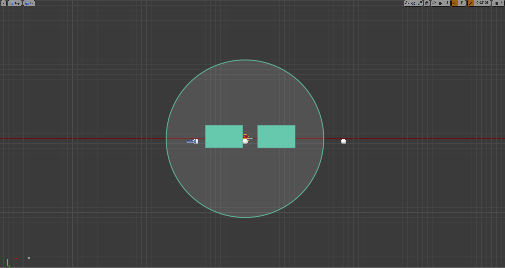
\includegraphics[width=0.8\textwidth]{movement}
\end{figure}

Se ha proporcionado la habilidad de salto para poder acceder a escenarios con diferentes alturas y dar al jugador una válvula de escape ante enemigos que puedan atosigarlo con múltiples proyectiles. El salto añade un movimiento repentino hacia arriba que hace posible esquivar proyectiles rápidos. 

\begin{figure}[H]
    \centering
    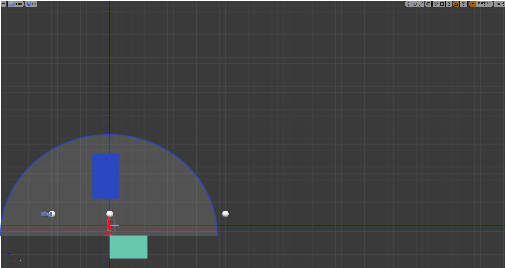
\includegraphics[width=0.8\textwidth]{movement_jump}
\end{figure}

El jugador puede moverse y cambiar de dirección instantáneamente a la misma velocidad que si estuviese en el suelo, por tanto tiene la misma zona de control horizontal en salto o moviéndose por el suelo. Se utiliza la gravedad por defecto de Unreal.

\section{Resource System}

\begin{figure}[H]
    \centering
    \includegraphics[width=1\textwidth]{resources_diagram}
\end{figure}

Definimos un recurso como una cantidad (float) que puede gastarse mientras esté sobre 0 y que tiene un máximo que puede almacenarse. La cualidad y comportamiento de \textit{ser un recurso} está definida en la interfaz \textit{\emph{ResourceBPInterface}} y el comportamiento básico de todos los recursos del juego queda descrito en el componente \textit{\emph{ResourceManagerCBP}}. Esta clase general nos permite modelar cualquier comportamiento que pueda tener un recurso derivándola a clases hijas con comportamientos más específicos, de ser necesario.

Un recurso tiene los siguientes parámetros:

\begin{description}
	\item[Max] Float. La cantidad máxima de recurso que se puede acumular.
	\item[Current] Float. La cantidad actual de recurso que el actor que posee el componente tiene.
\end{description}

Y los siguientes comportamientos, derivados de la interfaz:

\begin{description}
	\item[Refill()] Rellena el valor \textit{Current} del recurso hasta \textit{Max}.
	\item[Earn(Amount:Float)] Rellena el valor \textit{Current} en \textit{Amount} unidades sin sobrepasar \textit{Max}.
	\item[CanSpend(Amount:Float)] Devuelve un valor booleano \textit{True} si la cantidad especificada \textit{Amount} es mayor que la cantidad \textit{Current} de recurso, \textit{False} en caso contrario.
	\item[Spend(Amount:Float, Force: Boolean)] Decrementa \textit{Current} en \textit{Amount} unidades si \textit{CanSpend(Amount)} es \textit{True}. El parámetro \textit{Force} permite gastar dicha cantidad aunque \textit{CanSpend(Amount)} sea \textit{False} (dejando \textit{Current} en negativo).
\end{description}

\subsection{Health Manager}

El sistema de salud se basa en un recurso, implementado en \textit{\emph{HealthManagerCBP}}, que para ser más fácilmente identificable implementa la interfaz \textit{\emph{DamageableBPInterface}}\footnote{Esta misma interfaz es implementada por los jugadores y cualquier elemento que sea dañable. En el caso de los jugadores la implementación delega en un HealthManagerCBP su funcionamiento, después de generar los efectos de feedback al jugador dentro de su propia implementación. Al tener jugadores y componente la misma interfaz conectarlos es trivial.} y delega las funciones ReceiveDamage y WillDieIfDamaged al sistema de recursos.

El recurso pone a disposición del usuario 2 eventos que nos permiten implementar comportamiento relativo a ellos en otros Blueprints:

\begin{description}
	\item[OnDamageReceived] Se lanza este evento siempre que se llame a ReceiveDamage(), inmediatamente después de aplicar los efectos del daño.
	\item[OnDie] Si el resultado de ReceiveDamage() resulta en la muerte del jugador ($Current <= 0$), se lanza este evento inmediatamente después de aplicar los efectos del daño.
\end{description}

Sería muy fácil añadir una regeneración de salud por tiempo si se desease, como en el siguiente recurso (Maná), pero de momento se ha descartado para evitar que los jugadores alarguen la partida innecesariamente jugando a esconderse de sus enemigos y así favorecer el juego ofensivo.

\subsection{Mana Manager}

De forma similar al sistema de salud, el sistema de Maná en \textit{\emph{ManaManagerCBP}} implementa su propia interfaz \textit{\emph{UsesManaBPInterface}} que nos permite diferenciar actores que usan maná, como los jugadores. No implementa eventos propios, aunque en futuras iteraciones puede seguirse esta estrategia para acoplar efectos a los gastos y recuperaciones de maná. Sí implementa un atributo propio:

\begin{description}
	\item[ManaRechargePerSecond] Float. La cantidad de maná que se recupera por segundo, gestionado en el \textit{Event Tick} del componente.
\end{description}

La cantidad y regeneración de maná se ha pensado como un límite duro en la cantidad de hechizos que se pueden utilizar en un sólo asalto, pero que se regenera rápido para mantener una tensión constante entre poder provocar daño y tener que evitarlo.

\section{Magic System}

\begin{figure}[H]
    \centering
    \includegraphics[width=1\textwidth]{magic_system}
\end{figure}

\textit{\emph{MagicArsenalCBP}} es un componente que coordina todas las entidades que pueden usar hechizos con su arsenal de hechizos, ocupándose de gestionar los sistemas de disparo de hechizos, gasto de maná y cooldowns. Esta clase spawnea un \textit{\emph{SpellManagerBP}} para cada hechizo en su parámetro \textit{Spells} con el coste de maná y cooldown configurados, más un hechizo extra de utilidad de uso directo y cuenta con 2 funciones: Seleccionar un hechizo del arsenal y lanzarlo. La función de lanzar hechizo devuelve al actor que la haya usado el resultado del lanzamiento, un actor del tipo \textit{\emph{SpellBP}} o sus subclases y un valor de \textit{\emph{SpellFireResultEnumBP}}:

\begin{description}
	\item[SPELL\textunderscore FIRED] Todo correcto, el hechizo retornado puede usarse según el ciclo de vida explicado abajo.
	\item[CANT\textunderscore CAST\textunderscore NOT\textunderscore A\textunderscore MAGE] No se ha podido crear un hechizo porque el usuario no es un mago (no implementa \textit{\emph{UsesManaBPInterface}})
	\item[NOT\textunderscore ENOUGH\textunderscore MANA] El usuario no tiene suficiente maná para spawnear el hechizo.
	\item[STILL\textunderscore IN\textunderscore COOLDOWN] El hechizo está en tiempo de cooldown. El CD de cada hechizo cuenta desde el momento en el que éste se activa.
	\item[DOES\textunderscore NOT\textunderscore HAVE\textunderscore SPELL] Por causa de algún otro error (i.e. se ha intentado spawnear un hechizo que el manager no tiene) el hechizo no se ha spawneado. También ocurre si el actor que representa el hechizo no es válido en el momento de ser spawneado, por algún error interno, para poder fallar con seguridad.
\end{description}

\subsection{Spell Architecture}

Con éste sistema, las únicas responsabilidades de las clases que usan los hechizos son:

\begin{enumerate}
	\item Crear el hechizo usando las funcionalidades de su MagicArsenalCBP
	\item Llamar al evento \textit{Shoot(Target, ScaleVelocity)} en el momento correcto
\end{enumerate}

Todos los hechizos, con la clase base \textit{\emph{SpellBP}}, sean del tipo que sean, implementan un sistema de eventos que ligan el comportamiento del hechizo durante su ciclo de vida. Cada subclase; esto es, cada hechizo concreto; es responsable de llamar al evento correcto en el tiempo necesario:

\begin{description}
	\item[BeforeShooting] Por defecto se llama en el momento de crear el hechizo, sirve para crear efectos que se usan antes de disparar el hechizo.
	\item[ConsumeMana]\footnote{Debido a una limitación del motor (no es posible pasar callbacks como parámetro en la creación de objetos) debe asegurarse que ConsumeMana y SpellReady son llamados al menos en el frame siguiente de la creación, utilizando un Delay o una Timeline.} Activa las callbacks de consumir maná en la cadena de creación del hechizo ($SpellBP > SpellManagerBP > MagicArsenalCBP > Character$)\footnote{Toda esta ligadura utiliza el parámetro interno de los actores de Unreal \textit{Instigator}, que es el \textit{\emph{Character}} que ha creado toda la cadena en todos los objetos, es decir, el mago en cuestión.}.
	\item[SpellReady] Pasa el hechizo al estado SPELL\textunderscore READY. Activa las callbacks de hechizo listo para ser disparado en la cadena de creación del hechizo ($SpellBP > SpellManagerBP > MagicArsenalCBP > Character$).
	\item[AfterShooting] Inmediatamente después de activar el evento \textit{Shoot}, para activar efectos que deben ocurrir al lanzar el hechizo.
\end{description}

\subsection{Followers}

Los hechizos tienen un componente asociado del tipo \textit{\emph{FollowerCBP}}, que símplemente permite configurar hechizos para que se sitúen constantemente en una posición relativa al mago. Ésto nos sirve para crear bolas de fuego que siguen al mago hasta que son lanzadas, por ejemplo, un efecto fácil de implementar y que hace sentirse poderoso al lanzador. Como componentes que son pueden activarse y desactivarse cuando sea oportuno, y tienen las siguientes variables de configuración:

\begin{description}
	\item[Offset] Vector3D. Un vector en espacio local al creador del hechizo.
	\item[ApproximationPerSecond] Float. La proporción de trayecto entre la posición actual del hechizo y su posición necesaria de acuerdo a \textit{Offset} recorrida en un segundo.
	\begin{align}
		ApproximationPerSecond = 5.0
	\end{align}
	Esto significa que el hechizo en cuestión debería alcanzar una posición offset estática en 200ms desde donde sea que esté.
\end{description}

\subsection{Targets}

La interfaz \textit{\emph{TargetableBPInterface}} marca un actor como posible \textit{Target} de un hechizo, y permite al hechizo sacar cierta información del mismo sin comprometer otros datos del objeto, dándonos flexibilidad para hacer objetos que puedan ser afectados por hechizos rápidamente. Nominalmente la información más importante que se puede extraer de esta interfaz es la \textit{posición} del objetivo y el \textit{factor de gravedad} para hechizos con homing.

\subsection{Spell Projectiles}

Un \textit{\emph{SpellProjectileBP}} especializa la arquitectura de \textit{\emph{SpellBP}} para su uso en proyectiles, para ello añade una \textit{StaticMesh} sin colisión que representa el proyectil en pantalla, una \textit{SphereCollision} que describe el área de impacto que activa el proyectil y un \textit{ProjectileMovementComponent} estándar de Unreal que describe su movimiento. Describimos su comportamiento a continuación.

\subsubsection{MagicProjectileCollision Life Cycle}

\begin{figure}[H]
    \centering
    \includegraphics[width=1\textwidth]{fireball_ready_to_launch}
	\captionsetup{labelformat=empty}
    \caption{Aquí podemos ver la preparación de una bola de fuego para ser lanzada, con la colisión resaltada en amarillo.}
\end{figure}

La colisión de un projectil, a menos que se sobreescriba, es del tipo \textit{MagicProjectile}: overlap con el enemigo y con los objetos del mundo. Sin embargo, para evitar que el jugador destruya su propio proyectil caminando cerca de los muros éste canal de colisión se desactiva mientras el proyectil no se lanza (Event \textit{Shoot})\footnote{Sí se ha dejado que colisione contra jugadores, siendo posible spawnear un hechizo sobre otro jugador para dañarlo: ésto funciona bien porque el otro jugador puede hacer lo mismo, por tanto es una maniobra arriesgada pero posible.}. El proyectil spawnea una \textit{ExplosionBP} del tipo marcado en su atributo \textit{ExplosionPerStateOverride} según en el estado en el que esté, si ésta existe, o en caso contrario una \textit{ExplosionAtImpactDefault} al overlapear con cualquier objeto.

\subsubsection{Projectile Movement}

\begin{figure}[H]
    \centering
    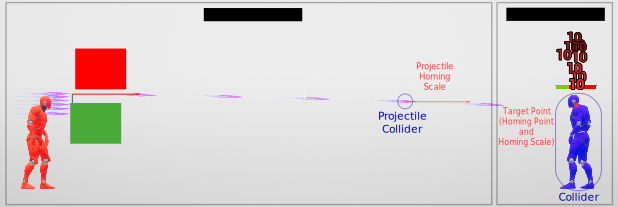
\includegraphics[width=1\textwidth]{projectiles_explained}
	\captionsetup{labelformat=empty}
    \caption{Un salvo de misiles mágicos con sus atributos de colisión y movimiento resaltados}
\end{figure}

El movimiento del proyectil se configura con 3 atributos principales:

\begin{description}
	\item[InitialVelocityScaling] Vector3D. Da la velocidad base de un hechizo en estado READY hacia el objetivo. Todos los proyectiles disparados con Shoot(Target, ScaleVelocity), por defecto se dirigen directamente hacia Target, con el vector director escalado por $InitialVelocityScaling * ScaleVelocity$\footnote{Esto sirve para aplicar distorsiones basadas en el movimiento del jugador (ver \textit{MainPlayerBP}) que hacen que los hechizos parezcan mejor apuntados. Al lanzarlos sin distorsión daba la sensación de que los hechizos quedaban sueltos en el aire detrás del jugador, gracias a este efecto ya no ocurre y los hechizos siguen funcionando igual.}.
	\item[GravityScale] Float. Siendo la gravedad de Unreal base una aceleración $[0.0, 0.0, -980.0]$ este valor escala dicho vector internamente al proyectil, siendo posible crear proyectiles con diferentes parábolas usando este parámetro y el anterior.
	\item[HomingAccelMagMultiplier] Este valor escala la ``gravedad'' entre el proyectil y el Target point seleccionado. El Target point tiene su propio valor de escala de gravedad, y combinando éstos dos parámetros pueden hacerse proyectiles con cualquier formato de homing, así como escalar lo que afecta el homing a cada objetivo.
\end{description}

\subsection{Explosions}

Una explosión es símplemente una \textit{SphereCollision} que aplica unos determinados efectos \textit{ApplyEffects(Actor)} \textbf{una única vez} a todos los actores con los que overlapee durante 0.2 segundos, para autodestruírse en ese momento. Con éste comportamiento, símplemente overrideando la función \textit{ApplyEffects}, y una visualización con efectos de partículas se realizan todos los efectos de los proyectiles presentes en el \textit{Vertical Slice}, la Fireball y el Magic Missile.

\subsection{Ad Hoc Solutions}

Se explican aquí elementos de juego que no utilizan completamente el sistema de hechizos para su funcionamiento y cómo.

\subsubsection{Circle of Fire}

El círculo de fuego \textit{CircleOfFireBP} utiliza un actor propio que crea colliders del tipo \textit{MagicProjectile} y aplica daño por segundo en cada tick a todos los actores con los que overlapee. El hechizo que lo spawnea \textit{SpellSpawnCircleOfFireBP} es subclase de \textit{SpellBP} estándar.

\subsubsection{Traps/Explosive Barrels}

\textit{No usado en Vertical Slice}. Las trampas son elementos del escenario (p.ej. barriles) que explotan en cuanto un hechizo o personaje los overlapea, haciendo daño a su alrededor. Para ello utilizan un preset de colisión específico \textit{ExplosiveBarrel} que spawnea la explosión del barril adecuada al ser overlapeado.

\subsection{Spell Library}

Describimos aquí la colección de hechizos disponibles en el \textit{Vertical Slice}:

\subsubsection{Fireball}

\begin{description}
	\item[Attributes] Projectile
	\item[Mana Cost] 30MP por uso
	\item[Damage] 200HP en el radio de explosión \textit{ExplosionDamagingFireballBP} (radius 2m)
	\item[Projectile Amount] 1
	\item[Prep Time] 1.2s
	\item[Cooldown] 5s
\end{description}

\begin{figure}[H]
    \centering
    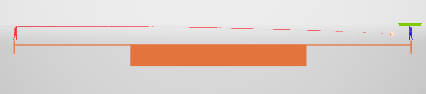
\includegraphics[width=1\textwidth]{fireball_trajectory}
\end{figure}

El hechizo básico, causa una gran cantidad de daño en área y tiene un área de control grande (se mueve rápidamente), pero necesita ser preparado durante un tiempo (1.2s) para ser efectivo. Si es disparado sin estar preparado desaparece en una explosión de humo. Se señala al jugador que el hechizo está preparado mediante una intensificación de los efectos de luz en el proyectil y el paso de efectos de partículas de humo a llamas.

\begin{figure}[H]
    \centering
    \includegraphics[width=1\textwidth]{fireball_timelines}
	\captionsetup{labelformat=empty}
    \caption{Aquí señalamos los eventos principales en el ciclo de vida de la Fireball, nótese la curva de intensidad con el pico en el momento en el que el hechizo se activa.}
\end{figure}

Se ha modelado éste hechizo sobre la gravedad base de Unreal, usándolo como base de pruebas para todos los hechizos, y en concreto para conseguir la sensación de peso y poder necesarias para que el juego fuese espectacular. El uso de una mesh que da sensación pesada y efectos de partículas que reflejen el comportamiento de la bola se ha prototipado con intención de servir de modelo a trabajo de arte real.

\textbf{Referencias:}

\href{https://www.gamasutra.com/view/news/271708/A_brief_history_of_the_fireball_in_fantasy_games.php}{Gamasutra - A brief history of the fireball in fantasy games}\footnote{\url{https://www.gamasutra.com/view/news/271708/A_brief_history_of_the_fireball_in_fantasy_games.php}}

\begin{figure}[H]
    \centering
    \includegraphics[width=1\textwidth]{great_chaos_fireball}
	\captionsetup{labelformat=empty}
    \caption{Great Chaos Fireball, \textit{Dark Souls} (2011)}
\end{figure}

\begin{figure}[H]
    \centering
    \includegraphics[width=1\textwidth]{fireball_wow}
	\captionsetup{labelformat=empty}
    \caption{Fireball, \textit{World of Warcraft} (2004)}
\end{figure}

\newpage
\subsubsection{Magic Missile}

\begin{description}
	\item[Attributes] Spawn Spell, Projectile
	\item[Mana Cost] 30MP por uso
	\item[Damage] 10HP por proyectil en un pequeño rango de explosión \textit{ExplosionDamagingMagicMissileBP} (radius 30cm)
	\item[Projectile Amount] 20
	\item[Prep Time] 0s
	\item[Cooldown] 1s
\end{description}

Un hechizo de disparo instantáneo que permite hacer gran cantidad de daño en poco tiempo, pero es difícil de apuntar a enemigos a distancias largas, pues es un hechizo lento. Consiste en crear un arco de prismas mágicos y lanzarlos en sucesión hacia el objetivo.

\textbf{Referencias:\footnote{\url{https://www.youtube.com/watch?v=gZDyejSNN54}}}
 
\begin{figure}[H]
    \centering
    \includegraphics[width=1\textwidth]{arcane_missiles_wow}
	\captionsetup{labelformat=empty}
    \caption{Arcane Missiles, \textit{World of Warcraft} (2004))}
\end{figure}

\begin{figure}[H]
    \centering
    \includegraphics[width=1\textwidth]{homing_soulmass_dark_souls}
	\captionsetup{labelformat=empty}
    \caption{Homing Soulmass, \textit{Dark Souls III} (2016)}
\end{figure}

\newpage
\subsubsection{Circle of Fire}

\begin{description}
	\item[Attributes] Spawn Spell
	\item[Mana Cost] 50MP por uso
	\item[Damage] 100HP/s mientras se esté en el área de efecto (franja de radio medio 400cm alrededor del objetivo, 180cm de ancho, 300cm de alto)
	\item[Cooldown] 10s
\end{description}

Como una de las mejores maneras de combatir consiste en moverse rápidamente para esquivar los hechizos es necesario un mecanismo que contrarreste esta estrategia. Por tanto, este hechizo conjura un círculo de fuego alrededor del objetivo para obligarle a decidir si recibe el daño moviéndose a través de él o se queda quieto y se expone a los hechizos de su contrincante.

\begin{figure}[H]
    \centering
    \includegraphics[width=0.5\textwidth]{circle_of_fire_config}
	\captionsetup{labelformat=empty}
    \caption{Configuración del círculo generado en el punto de impacto.}
\end{figure}

\begin{figure}[H]
    \centering
    \includegraphics[width=0.6\textwidth]{circle_of_fire_procedural}
	\captionsetup{labelformat=empty}
    \caption{El círculo de fuego generado.}
\end{figure}

La clase responsable de crear el círculo es \textit{SpellSpawnCircleOfFireBP}, que es del tipo \textit{SpellBP}. El proceso es el siguiente:

\begin{enumerate}
	\item Raytrace entre el lanzador y el objetivo. Se obtiene una posición según:
	\begin{enumerate}
		\item Si el raytrace falla (el objetivo está demasiado lejos, o estamos utilizando el objetivo que tiene el personaje propio para apuntar hacia adelante) se utiliza la posición del objetivo
		\item En otro caso utilizamos el punto de impacto del raytrace.
	\end{enumerate}
	\item Desde esta posición realizamos un raytrace al suelo, donde se spawnea el círculo de llamas.
\end{enumerate}

Mientras el hechizo no se dispara se spawnea un \textit{FakeCircleOfFireBP} que sólo contiene representación gráfica para informar al jugador del lugar donde se lanzará el hechizo.

\textbf{Referencias:}

\begin{figure}[H]
    \centering
    \includegraphics[width=1\textwidth]{ring_of_fire_wow_reference}
	\captionsetup{labelformat=empty}
    \caption{Ring of fire (visual reference), \textit{World of Warcraft} (2004)}
\end{figure}

\newpage
\subsubsection{Magic Shield}

\begin{description}
	\item[Attributes] Normal Spell
	\item[Mana Cost] 20MP cada 0.5s, desactivable
	\item[Cooldown] 0s
\end{description}

El escudo mágico es un \textit{hechizo de utilidad} que permite a un jugador hacer que su oponente gaste sus recursos inútilmente, añadiendo un nivel extra de \textit{mindgames} al juego. El hechizo gasta mucho maná, pero hace que todo el daño que el jugador reciba quede anulado y convierte un 10\% del daño en maná extra para el usuario. Por tanto es un hechizo útil para tentar al contrario a lanzar un ataque y responder con fuerza en el momento en el que sus reservas de maná están bajas.

\textbf{Referencias:}

\begin{figure}[H]
    \centering
    \includegraphics[width=1\textwidth]{anti_magic_shield_wow}
	\captionsetup{labelformat=empty}
    \caption{Anti-magic Shield, \textit{World of Warcraft} (2004)}
\end{figure}

\section{Sound Management System}

Todos los sonidos utilizan la función \textit{PlaySound} del componente \textit{\emph{SoundEffectsManagerCBP}} directamente, que a su vez utiliza los componentes propios de Unreal. Extender esta clase nos permite mantener todos los sonidos que genera un objeto encapsulados en un objeto, para evitar añadir complejidad en otros componentes. De la misma forma se usa una subclase de éste, \textit{\emph{DelegateToInstigatorSoundEffectsManagerBP}}, para delegar el manejo de sonidos en hechizos a su creador. De ésta manera se parten las responsabilidades entre hechizo e instigador permitiendo modificarlos según la lógica del hechizo pero pudiendo persistir más allá de su ciclo de vida.

\section{Levels}

\subsection{Level Design Principles}

Para el modo de juego \textit{Aniquilación}:

\begin{itemize}
	\item Los jugadores han de poder verse desde el principio del juego, resaltando que el juego es un ``duelo''
	\item Estructura simple: cada jugador debe poder saber las posibilidades de movimiento que él mismo y su contrincante tienen
	\item Estructuras defensivas: debe ser fácil hacer movimientos que pongan una estructura entre tú y tu enemigo, como maniobra defensiva
	\item Escaso movimiento vertical: Dado que las mecánicas de movimiento vertical son limitadas, no debe ponerse el énfasis en el movimiento vertical.\footnote{La táctica se enfoca sobre el movimiento sobre el plano horizontal, que tiene un espacio de posibilidades lo suficientemente grande como para tener profundidad. El movimiento vertical se utiliza nada más como válvula de escape para el jugador, como se explica en la sección sobre controles.}
\end{itemize}

\subsection{The Sphere of Lyra}

\begin{figure}[H]
    \centering
    \includegraphics[width=0.8\textwidth]{sphere_of_lyra_0}
\end{figure}

La Esfera de Lyra es un artefacto de inmenso poder, capaz de conceder cualquier deseo que un mago pueda tener, sin embargo no está libre de consecuencias. Cualquier mago puede utilizarla, pero al hacerlo se verá obligado a cargar con la esfera por el resto de su vida, esto es, hasta que otro mago quiera conseguirla. La esfera obliga al poseedor y a quien quiera obtenerla a luchar por ella en un universo de bolsillo que al mismo tiempo la contiene y está delimitado por ella. Internamente se visualiza como un jardín en el que reposa esperando a ser obtenida por su siguiente propietario.

\textbf{Level Structure:}

\begin{figure}[h]
    \centering
    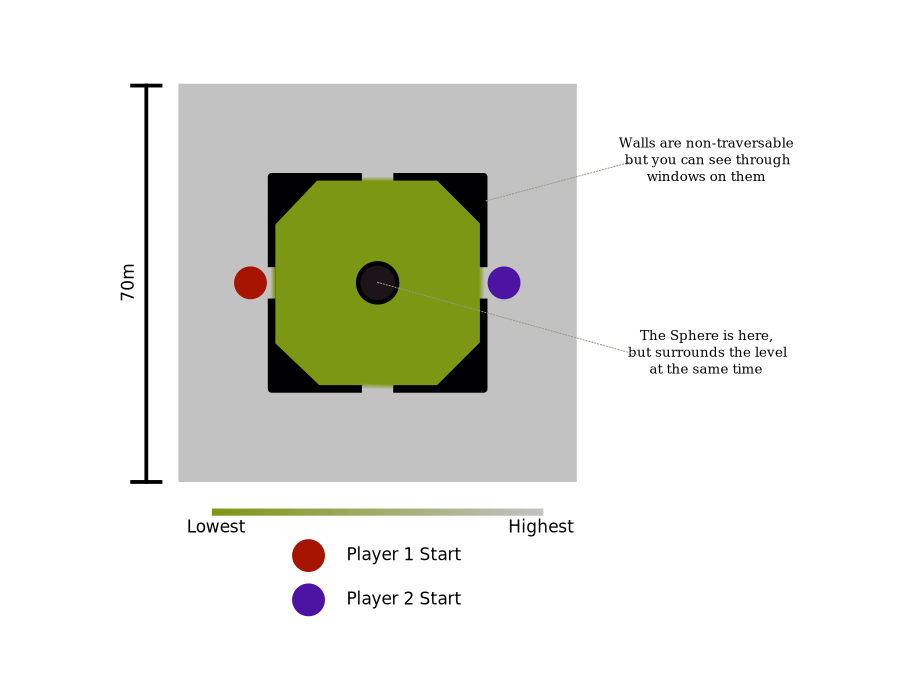
\includegraphics[width=1.2\textwidth]{sphere_of_lyra_map}
\end{figure}

\newpage
\textbf{References:}

\begin{figure}[h]
    \centering
    \includegraphics[width=0.8\textwidth]{sphere_of_lyra_1}
\end{figure}

\begin{figure}[h]
    \centering
    \includegraphics[width=0.8\textwidth]{sphere_of_lyra_2}
\end{figure}

\begin{figure}[h]
    \centering
    \includegraphics[width=0.8\textwidth]{sphere_of_lyra_4}
\end{figure}

\begin{figure}[h]
    \centering
    \includegraphics[width=0.8\textwidth]{sphere_of_lyra_3}
\end{figure}

\section{AI Agents}

Describimos aquí los componentes de IA desarrollados.

\subsection{Enemy Example}

El \textit{\emph{EnemyExampleBP}} es un \textit{\emph{MainPlayerBP}} controlado por IA, usando \textit{\emph{EnemyExampleAIControllerBP}} con el árbol de comportamiento \textit{\emph{BTEnemyExample}}. La única modificación que tiene consiste en que su regeneración de maná es ligeramente más alta, para ayudar a mantener la presión sobre el jugador.

\begin{figure}[h]
    \centering
    \includegraphics[width=1\textwidth]{base_behavior_tree}
\end{figure}

En la raíz del arbol de comportamientos seleccionamos entre una estrategia agresiva o defensiva (implementadas cada una en su propio sub-árbol). Se escoge estrategia defensiva, por el momento, si el agente tiene menos de un 20\% de su salud total, y agresiva en caso contrario.

\begin{figure}[H]
    \centering
    \includegraphics[width=1\textwidth]{aggresive_behavior_tree}
\end{figure}

La estrategia agresiva consiste en mantener una presión constante sobre el enemigo sin dejarle respirar. Para ello se ejecutan, según prioridad, estas tareas:

\begin{enumerate}
	\item Si no podemos ver al enemigo (utilizando un raytrace rectangular, para dejar espacio para los disparos), nos movemos hacia él.
	\item Si no tenemos un hechizo preparado creamos uno nuevo y lo mantenemos
	\item Si podemos ver al enemigo
	\begin{enumerate}
		\item Disparamos continuamente
		\item Nos movemos continuamente para no ser alcanzados
	\end{enumerate}
\end{enumerate}

\begin{figure}[H]
    \centering
    \includegraphics[width=1\textwidth]{defensive_behavior_tree}
\end{figure}

La estrategia defensiva consiste en mantenerse a cubierto, lanzando hechizos mientras se huye para rechazar al enemigo si éste está a la vista.

Añadimos como detalles de implementación que no son completamente intuitivos a primera vista.

\begin{itemize}
	\item La implementación del nodo \textit{\emph{DHaveLineOfSightBTDecorator}} que determina si hay línea de visión entre 2 jugadores no se implementa con un raytrace simple, sino con un box trace, para permitir dejar espacio para disparar los hechizos que siguen a los jugadores con un offset (con \textit{FollowerCBP}).
	\item La implementación del nodo \textit{\emph{SFindNearbyPlaceToMoveBTService}}, que decide el siguiente punto del mapa al que moverse (para no parar de moverse), sigue el siguiente esquema:
	\begin{figure}[H]
	    \centering
	    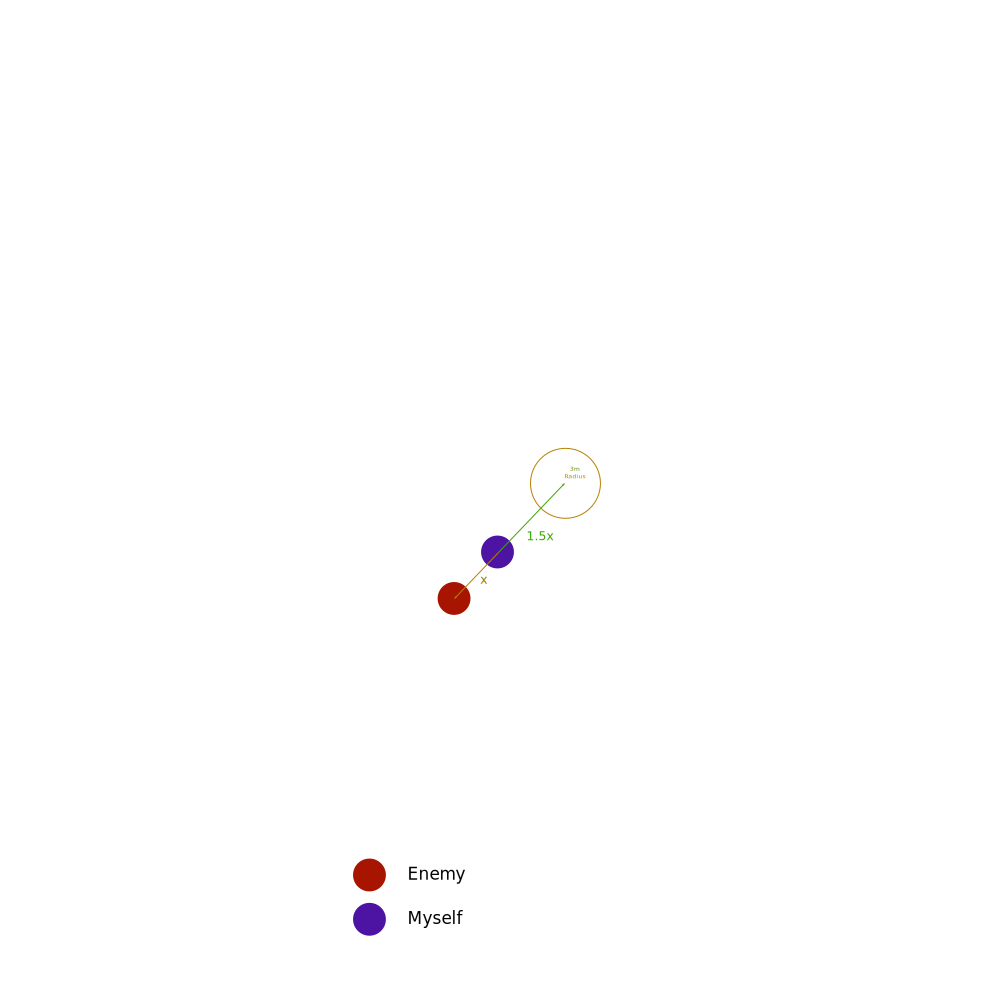
\includegraphics[width=1\textwidth]{positioning_scheme}
		\captionsetup{labelformat=empty}
	    \caption{Se selecciona un punto aleatorio dentro del círculo de 3 metros para ser el siguiente punto al que moverse, a partir de la posición del enemigo. Si no se está huyendo símplemente se considera $x = 0$ en el esquema anterior, i.e. alrededor del propio agente.}
	\end{figure}
\end{itemize}

\cleartoleftpage

\part{Business and Operations Design Notes}

\chapter{Monetization}

La esperanza de vida del juego queda definida como 10.000 jugadores online diarios, ó 7 jugadores concurrentes buscando partida por minuto, ó 1 partida formándose por minuto. Llegado este punto el juego online es claramente insostenible (demasiado tiempo de espera por una partida). Todo plan de negocio planteado para este juego ha de tener este dato en cuenta\footnote{Si el plan de negocio apunta a zonas horarias limitadas (no \textit{worldwide}) esta media puede bajarse siempre y cuando el principio ``1 partida por minuto'' se mantenga en las horas puntas de juego de dichas zonas.}. Para ello el juego debe ser constantemente rejugable y por tanto han de incluírse quests diarias para reclamar la atención regular del jugador combinado con un gameplay ajustado y dinámico: esto combina un coste variable continuo en el tiempo con la necesidad de insumos constantes para compensar dichos costes.

Todos los datos de juego (desbloqueos y personalización) se guardan en un sistema de servidores remoto que será accedido por el juego para matchmaking, esto aumenta los costes de mantenimiento del producto. Para costearlos se plantea un flujo de insumos proveniente de la venta de \textit{lootboxes} con contenido estético y nuevos elementos de jugabilidad (hechizos) para los personajes. A largo plazo puede extenderse a nuevos modos de juego o incluso campañas con foco narrativo que extiendan el universo de juego.

\chapter{Network}

Para garantizar la mejor experiencia de usuario a un coste bajo se utiliza una combinación de servicios mínimos para dar la información mínima a los clientes de juego para que gestionen partidas entre ellos, enviando de vuelta al servidor cada uno su copia local de la partida jugada para valoración anti-cheat. Como ejemplo, \textit{Raiders of the Broken Planet} utiliza un sistema de matchmaking similar a éste, siendo necesario el trabajo de matchmaking cross-platform para mantener unos niveles de jugadores concurrentes aceptables (para tiempos de matchmaking bajo).

\begin{figure}[h]
    \centering
    \includegraphics[width=0.6\textwidth]{network}
\end{figure}

\cleardoublepage

\thispagestyle{empty}

\vspace*{\fill}

\begin{figure}[h]
    \centering
    \includegraphics[width=0.6\textwidth]{fireball}
\end{figure}

\vfill

\end{document}
